
\documentclass[11pt]{article} 

\usepackage[utf8]{inputenc} 
\usepackage{geometry} 
\geometry{a4paper} 

\vspace{2cm}
\setlength{\parindent}{0cm}
\usepackage{graphicx,wrapfig,placeins}

\title{Interactive Graphics}
\author{Chichi Francesco, Jary Pomponi}

\begin{document}
\maketitle
\graphicspath{{img/}}

\section{List of all the libraries, tools and models used in the project but	not developed by the team}
\begin{itemize}
	\item \textbf{Three.js:}
		Three.js is a cross-browser JavaScript library/API used to create and display animated 3D computer graphics in a web browser exploiting the power of WebGL in an high level mode.
	\item \textbf{OrbitControls.js:}
	\item \textbf{Detector.js:}
	\item \textbf{stats.min.js:}
\end{itemize}
\section{Description of all the technical aspects of the project}
\subsection{Ship}
	
	
	\begin{wrapfigure}{R}{0pt}
		\centering
		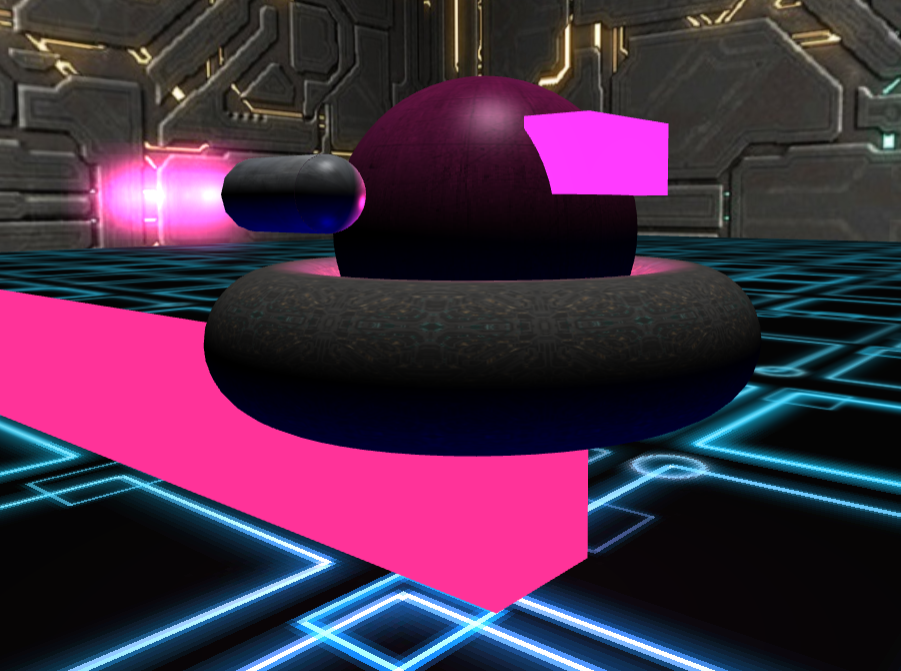
\includegraphics[width=0.4\linewidth]{ship}
		\caption{This is the character of a player that choosed the pink colour.}
		\label{fig:ship}
	\end{wrapfigure}
	
	Each player has a ship of the choosen colour, which one is a three.js Group, composed by a \textbf{cabin} (fig. 2), a clock wise rotating \textbf{ring} (fig. 3) and two \textbf{motors} (fig. 4).\\
	
	The cabin is also a Group of element coloured with the player's colour, composed by a glass and a cockpit with a pointlight inside.
	The cockpit is a sphere covered with a metallic texture, the glass is a parallelepiped made by a MeshToonMaterial, that is illuminated by the cockpit's light.\\
	
	Each motor is another independent Group, composed by a cylinder, an hemisphere on the top and another hemisphere with an hole, that represent the exhaust pipe, each one is covered with the metallic texture of the cabin.
	Furthermore, at the end of the exhaust pipe, there are 50 particles of the colour of the player. The wake's length where this particles are distributed is choosen stochastically: with a probability of 80\%, the wake's length is equal to 40, with 10\% is 0 or 10.\\
	
	Finally, there is a rotating ring, that is a torus coloured with the same texture of the torus which rotates around the map.
	
	\begin{figure}
		\centering
		\begin{minipage}[b]{0.25\linewidth}
			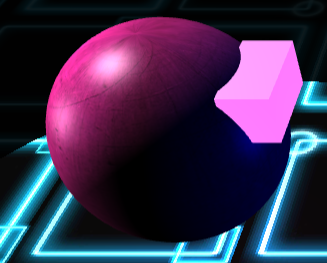
\includegraphics[width=\linewidth]{cabin}
			\caption{}
			\label{fig:cabin}
		\end{minipage}
		\begin{minipage}[b]{0.276\linewidth}
			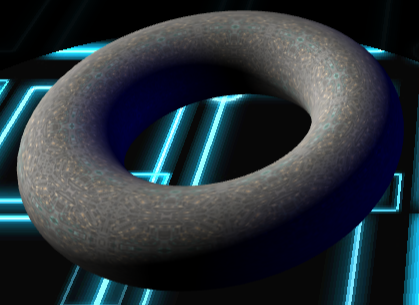
\includegraphics[width=\linewidth]{toro}
			\caption{}
			\label{fig:toro}
		\end{minipage}
		\begin{minipage}[b]{0.6\linewidth}
			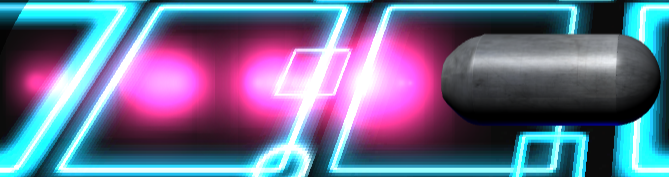
\includegraphics[width=\linewidth]{motor}
			\caption{}
			\label{fig:motor}
		\end{minipage}
	\end{figure}





\subsection{Halo}
\subsection{Animated Light}
\subsection{Collision}
\subsection{Menu}
\subsubsection{Kyeboard settings}
\subsubsection{Color settings}


\section{Description of the implemented interactions}

\end{document}
